\documentclass{beamer}
\usetheme{Boadilla}
\usepackage[utf8]{inputenc}
\usepackage{appendixnumberbeamer}
\setbeamercolor{alerted text}{fg=blue!150!black!100}  %

\usepackage[normalem]{ulem}

\newcommand\gagnerduTemps[1]{#1}


\definecolor{green}{rgb}{0.0, 0.6, 0.0}
\definecolor{red}{rgb}{0.7, 0.0, 0.0}
\definecolor{blue}{rgb}{0.0, 0.0, 0.8}
\beamertemplatenavigationsymbolsempty
\usepackage{tikz}
\usepackage{appendixnumberbeamer}
\usetikzlibrary{shapes,arrows,positioning,automata}
\newcommand\object[1]{\node[fill] at (#1) {~};}

\everymath{\displaystyle}

\newcommand\mpage[2]{%
  \begin{minipage}{#1\linewidth}%
    #2%
  \end{minipage}%
}

%%%%%%%%%%%%%%%%%%%%%%%%%%%%%%%%%%%%%%%%%%%%%%%%%%%%%%%%%%%%%%%%%%%%%%%%
%%% The following black magic puts copies of the table of contents
%%% throughout your talk: you might not want this.
\AtBeginSection[]
{
  \begin{frame}{Outline}
    \tableofcontents[current,currentsection]
  \end{frame}
}
%%%%%%%%%%%%%%%%%%%%%%%%%%%%%%%%%%%%%%%%%%%%%%%%%%%%%%%%%%%%%%%%%%%%%%%%


\newcommand\dt{\frac{d}{dt}}
\newcommand\esp[1]{\mathbb{E}\left[#1\right]}
\newcommand\var[1]{\mathrm{var}\left[#1\right]}
\graphicspath{{figs/}{../simulations/output_pdfs/}{}}

\definecolor{violet}{rgb}{0.3, 0., 0.2}
\definecolor{darkgreen}{rgb}{0, 0.2, 0}
\definecolor{darkred}{rgb}{.4, 0, 0}
\definecolor{darkblue}{rgb}{0, 0, 0.5}
\setbeamercolor{math text}{fg=violet}
\newcommand\red[1]{{\color{red}#1}}
\newcommand\blue[1]{{\color{blue}#1}}
\newcommand\green[1]{{\color{green}#1}}
\newcommand\bx{\mathbf{x}}


\newcommand\bm{\mathbf{m}}
\newcommand\expect[1]{\mathbb{E}\left[#1\right]}
\newcommand\E{\mathbb{E}}
\newcommand\calS{\mathcal{S}}
\newcommand\calE{\mathcal{E}}
\newcommand\calA{\mathcal{A}}
\newcommand\calB{\mathcal{B}}
\newcommand\calT{\mathcal{T}}
\newcommand\calP{\mathcal{P}}
\newcommand\calL{\mathcal{L}}
\newcommand\Proba[1]{\mathbf{P}\left[#1\right]}
\newcommand\proba[1]{\mathbf{P}\left[#1\right]}
\newcommand\norm[1]{\left\|#1\right\|}
\newcommand\abs[1]{\left|#1\right|}
\newcommand\N{\mathbb{Z}^+}
\newcommand\R{\mathbb{R}}
\newcommand\bbm{\mathbf{m}}
\newcommand\bX{\mathbf{X}}
\newcommand\bE{\mathbf{E}}
\newcommand\LN{L^{(N)}}
\newcommand\bl{{\text{\boldmath$\ell$}}}

\DeclareMathOperator*{\argmin}{arg\,min}

\setbeamertemplate{blocks}[rounded][shadow=false]
\setbeamercolor*{block title}{fg=blue!70!black!90, bg=blue!8}
\setbeamercolor*{block body}{bg=blue!4}

\tikzset{every picture/.append style={shorten >=2pt,line width=2pt}}
\tikzstyle{wide}=[line width=2pt,->]

\makeatother
\setbeamertemplate{footline}
{
  \hfill 
  \usebeamerfont{author in head/foot}\insertshortauthor{} -- 
  \insertframenumber{} / \inserttotalframenumber\hspace*{1ex}
  \vskip0pt%
}
\makeatletter

\begin{document}

\title{Size Expansions of Mean Field Approximation: Transient and
  Steady-State Analysis}%
\author[Nicolas Gast]{
  \begin{tabular}{ccc}
    \textbf{Nicolas Gast}
    &Luca Bortolussi
    &Mirco Tribastone\\
    Inria, France
    & Univ. Trieste, Italy
    &IMT Lucca, Italy
  \end{tabular}
}
\institute[Inria, France]{}%
\date{IFIP Performance 2018, Toulouse}%

\maketitle

\begin{frame}{Good system design needs performance evaluation}
  {Example : load balancing}

  \begin{tabular}{cc}
    \mpage{.4}{
    \centering
    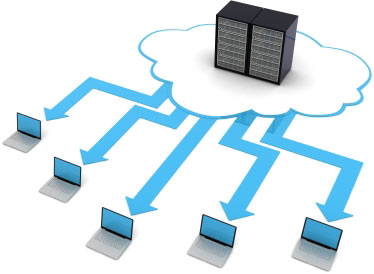
\includegraphics[width=\linewidth]{cluster-server}\\
    $N$ servers}
    &~~\mpage{.5}{
      Which allocation policy? 
      \begin{itemize}
      \item Random 
      \item Round-robin 
      \item $JSQ$
      \item $JSQ(d)$ 
      \item $JIQ$ 
      \end{itemize}
      }
  \end{tabular}
  \vspace{1cm}
  \pause
  
  We need methods to characterize emerging behavior starting from a
  stochastic model of interacting objects
  \begin{itemize}
  \item We can use \blue{mean field approximation}.
  \end{itemize}
\end{frame}

\begin{frame}{Mean Field and Refined Mean Field Approximations}
  For the steady-state performance of many systems,\footnote{{\tiny
      Ref: ``A Refined Mean Field Approximation'' by G. and Van Houdt
      (SIGMETRICS 2018)}}:
  \begin{align*}
    Perf(N) \approx
    \only<1>{\underbrace{Perf(\infty)}_{\text{mean field approximation}} +
    \qquad\frac{V}{N}\qquad}
    \only<2->{\underbrace{\underbrace{Perf(\infty)}_{\text{mean field approximation}} +
    \qquad\frac{V}{N}\qquad}_{\text{\color{darkgreen}refined mean field approximation}}}
  \end{align*}
  \only<1>{\vspace{.6cm}}
  
  We provided analytical and  numerical methods to compute $V$.
  \bigskip
  
  Example: steady-state average queue length ($\rho=0.9$)\bigskip
  
  \begin{tabular}{c|c|c|c|c|c}
    Policy & Mean Field ($N=\infty$)
    &\multicolumn{2}{c|}{$N=100$}
    &\multicolumn{2}{c|}{$N=10$}\\
           &&Simu. \uncover<2->{&R.M.F.}
    & Simu\uncover<2->{&R.M.F.} \\\hline
    SQ(2) & 2.35 & 2.39  \uncover<2->{&\color{darkgreen} 2.39}
      &2.80\uncover<2->{&\color{darkgreen}2.75}\\
    Pull-push & 1.64  & 1.70 \uncover<2->{&\color{darkgreen}1.70}
      & 2.30\uncover<2->{&\color{darkgreen}2.29}
  \end{tabular}
  
\end{frame}

\begin{frame}{ Question addressed in this work}
  
  \begin{exampleblock}{Our contributions}
    \begin{itemize}
    \item We can compute the next term in the expansion.
    \item We can do the same analysis for the transient regime?
    \item We study the cost (computation) and the benefit (accuracy).
    \end{itemize}
  \end{exampleblock}

  \begin{align*}
    Perf(N,t) \approx
    Perf(\infty,t)+\frac{V(t)}{N}+\frac{A(t)}{N^2}+\dots 
  \end{align*}
\end{frame}

\begin{frame}{Outline}
  \tableofcontents
\end{frame}

\section{Classical Mean Field Approximation}

\begin{frame}{``Mean field approximation'' simplifies many
    problem}{But how to apply it?}
  
  \begin{align*}
    \lim_{N\to\infty}\left(\begin{array}{c}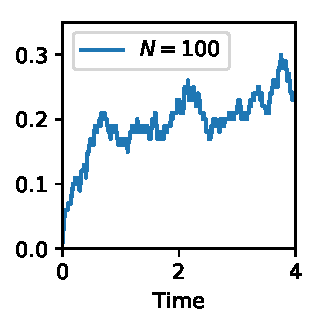
\includegraphics[width=.28\linewidth]{traj_rho80_onlyN100}\end{array}\right) 
    =\underbrace{\begin{array}{c}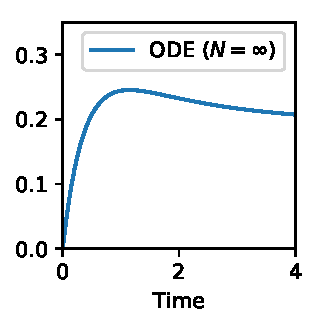
\includegraphics[width=.28\linewidth]{traj_rho80_onlyNinf}\end{array}}_{
    \text{Mean field approximation}}
  \end{align*}
  
  Applications : 
  \begin{itemize}
  \item Performance of load balancing / caching algorithms
  \item Communication protocols (CSMA, MPTCP, Simgrid)
  \item Mean field games (evacuation, Mexican wave)
  \item Stochastic approximation / learning 
  \item Theoretical biology 
  \end{itemize}
\end{frame}

\begin{frame}{The supermarket model (SQ(2))}
  \begin{tabular}{@{}cc}
    \mpage{.6}{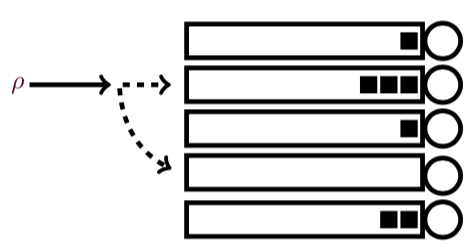
\includegraphics[width=\linewidth]{supermarket}}
    &\mpage{.35}{Arrival at each server $\rho$.
      \begin{itemize}
      \item Sample $d-1$ other queues. 
      \item Allocate to the shortest queue
      \end{itemize}
      Service rate=$1$.
      }
  \end{tabular}
\end{frame}

\begin{frame}{$SQ(d)$: state representation}
    The state space is $X=(X_1,X_2,\dots)$ where
    \begin{align*}
      X_i(t) = \text{\blue{fraction of queues with queue length $\ge
      i$}.} 
    \end{align*}
  \bigskip
  
  \begin{tabular}{cc}
    \mpage{.3}{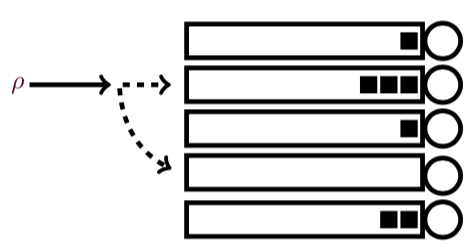
\includegraphics[width=\linewidth]{supermarket}}
    &\mpage{.6}{$X=(1,0.8,0.4,0.2,0,0,0,\dots)$}
  \end{tabular}


\end{frame}


\begin{frame}{State transitions and Mean Field Approximation}
  State changes on $x$:
  \begin{align*}
    x\mapsto x + \frac1N\mathbf{e_i} & \text{ at rate $N\rho(x_{i-1}^d-x_{i}^d)$}\\
    x\mapsto x - \frac1N\mathbf{e_i} & \text{ at rate $N(x_i-x_{i+1})$}\\
  \end{align*}

  The mean field approximation is to consider the ODE associated with
  the drift (average variation):
  \begin{align*}
    \dot{x}_i = \underbrace{\rho(x_{i-1}^d-x_{i}^d)}_{\mathrm{Arrival}}
    -\underbrace{(x_i-x_{i+1})}_{\mathrm{Departure}}
  \end{align*}
\end{frame}

\begin{frame}{Density dependent population process (Kurtz, 70s)}
  A population process is a sequence of CTMCs $X^N(t)$ indexed by the
  population size $N$, with state space $E^N\subset E$ and
  transitions (for $\ell\in\calL$): 
  \begin{align*}
    X \mapsto X+\frac{\ell}{N} \qquad \text{ at rate
    $N\beta_\ell(X)$}.
  \end{align*}
  \pause
  
  \begin{center}
    \mpage{.9}{
      \begin{exampleblock}{The Mean field approximation}
        The \alert{drift} is
        $\displaystyle f(x) = \frac{d}{dt}\esp{X(t)\mid
          X(0)=x}=\sum_{\ell} \ell \beta_\ell(x)$.\\
        The mean field approximation is the solution of the ODE
        $\dot{x}=f(x)$.
      \end{exampleblock}
    }
  \end{center}
  \bigskip\pause
  \alert{Example}: SQ(d) load balancing
  \begin{align*}
    \dot{x}_i = \rho(x_{i-1}^d - x_i^d) - (x_i-x_{i+1})
  \end{align*}
  It has a unique attractor: $\pi_i=\rho^{(d^i-1)/(d-1)}$. 
\end{frame}

\begin{frame}{Accuracy of the mean field approximation}
  {Numerical example of SQ($d$) load balancing ($d=2$)}

  \begin{tikzpicture}
    \node at (0,0){
    \begin{tabular}{@{}c|ccccc|c}
      & \multicolumn{5}{c|}{Simulation (steady-state average queue
        length)}&Fixed Point\\ 
      N &  10&20&30&50&100&$\infty$ (mean field)\\\hline
    $\rho = 0.7$&1.2194&1.1735&1.1584&1.1471&1.1384&1.1301\\\hline\hline
    $\rho = 0.9$&2.8040&2.5665&2.4907&2.4344&2.3931&2.3527\\\hline\hline
    $\rho=0.95$&4.2952&3.7160&3.5348&3.4002&3.3047&3.2139\\\hline\hline
    \end{tabular}
  };
  \only<2>{\draw[darkgreen,dashed] (1.5,-1.2) rectangle (6,0.9);}
      \end{tikzpicture}

  \bigskip
  
  \alert{Fairly good accuracy for $N=100$ servers.}
\end{frame}

\section{System Size Expansion}

\begin{frame}{Expected values estimated by mean field are
    1/N-accurate}

    Some experiments (for SQ(2) with $\rho = 0.9$):
  \begin{tabular}{c|ccc|c}
    $N$&$10$&$100$&$1000$&$\infty$\\\hline
    Average queue length (simulation)&
    2.8040 &2.3931 &2.3567&2.3527\\ 
    Error of mean field &0.4513&0.0404&0.0040&0
  \end{tabular}
  
  \alert{Error decreases as $1/N$}
\end{frame}

\begin{frame}{Where does the $O(1/N)$-term comes from?}

  For $SQ(2)$: The transitions on $X_i$: $+\frac1N$ at rate
  $N(x_{i-1}^2-x_i^2)$ and $ -\frac1N$ at rate $N(x_{i}-x_{i+1})$.
  Hence:
  \begin{align*}
    \dt \esp{X_i(t)}
    =\esp{X_{i-1}^2(t)-X_i^2(t)-(X_{i}(t)-X_{i+1}(t))}
    &\text{\quad\color{blue}(exact)}\\ 
    =\esp{X_{i-1}^2(t)}-\esp{X_i^2(t)}-\esp{X_{i}(t)}+\esp{X_{i+1}(t)}\\
    \uncover<2->{\text{\only<3->{\sout}{$\displaystyle\blue{\approx}
    \esp{X_{i-1}(t)}^{\blue{2}}-\esp{X_i(t)}^{\blue{2}}-\esp{X_{i}(t)}+\esp{X_{i+1}(t)}$}} 
    &{\text{\quad\color{blue}(mean field approx.)}}}
  \end{align*}\pause\pause
  If we now consider how $\esp{X_i^2}$ evolves, we have: 
  \begin{align*}
    \dt \esp{X_i^2} &= \esp{(2X_i+\frac1{N})(X_{i-1}^2-X_i^2)
                      + (-2X_i+\frac1{N})(X_{i}-X_{i+1})}\\
                    &=\esp{
                      \underbrace{2X_iX_{i-1}^2}_{\blue{\esp{X_iX_{i-1}^2\approx
                      ?}}} + \dots\dots\dots\dots}
  \end{align*}
  where we denote $X$ instead of $X(t)$ for simplicity. 
\end{frame}

\begin{frame}{System Size Expansion Approach}
  Recall that the transitions are $X\mapsto X+\frac\ell N$ at rate
  $N\beta_\ell(x)$. 
  \begin{align*}
    \dt \esp{X} &= \esp{\sum_{\ell}\beta_\ell(X)\ell} =
    \esp{f(X)} && \text{ \blue{(Exact)}}\\
    \dt x &= f(x) && \text{ \blue{(Mean Field Approx.)}}
  \end{align*}\pause
  We can now look at the second moment:
  \begin{align*}
    \esp{(X-x)\otimes(X-x)}
    &=\esp{(f(X)-f(x))\otimes (X-x)} &\text{\blue{(Exact)}}\\
    &\quad+\esp{(X-x)\otimes(f(X)-f(x))}\\
    &\quad+\frac1N\esp{\sum_{\ell\in\calL}\beta_\ell(X)\ell\otimes\ell}
  \end{align*}
  \pause
  ... We can also look at higher order moments
  \begin{align*}
    &\esp{(X-x)^{\otimes3}}
    =3\mathrm{Sym}\esp{(f(X)-f(x))\otimes(X-x)\otimes(X-x)}\\
    &\qquad+\frac3N\mathrm{Sym}\esp{\sum_{\ell\in\calL}\beta_\ell(X)\ell\otimes\ell\otimes(X-x)}+\frac1N\esp{\sum_{\ell\in\calL}\beta_\ell(X)\ell\otimes\ell\otimes\ell}
  \end{align*}
\end{frame}

\begin{frame}{Using this approach, we can derive linear ODEs}
  \textbf{Theorem.} Assume that $f$ is $C^{2}$ and let $x$ be the
  solution of $\dt x = f(x)$.
  \begin{align*}
    \dt{\esp{X(t)}} &= x(t) + O(1/N).
  \end{align*}\pause 
  \footnotesize Let $Y(t)=X(t)-x(t)$. Then :
  \begin{align*}
    \esp{Y(t)} &= \frac1NV(t)+\only<2>{O(1/N^2)}\only<3>{{\color{red}\frac1{N^2}A(t)} + O(1/N^{\color{red}3})}\\
    \esp{Y(t)\otimes Y(t)}&=\frac1NW(t)+\only<2>{O(1/N^2)}\only<3>{{\color{red}\frac1{N^2}B(t)} + O(1/N^{\color{red}3})}\uncover<3>{\\
    \color{red}esp{Y(t)^{\otimes3}}&\color{red}=\frac1{N^2}C(t) + O(1/N^3)\qquad\qquad\\
    \color{red}esp{Y(t)^{\otimes4}}&=\color{red}\frac1{N^2}D(t) + O(1/N^3)}
  \end{align*}
  where \only<3>{\tiny}
  \begin{align*}
    \dt V^i &= f^{i}_j V^j + f^{i}_{j,k} W^{j,k}\\
    \dt W^{j,k} &= f^{j}_\ell W^{\ell,k} + f^{k}_\ell W^{j,\ell}\\
    \uncover<3->{\dt A^i &= f^i_j A^j + f^{i}_{j,k}B^{j,k} +
                           f^{i}_{j,k,\ell}C^{j,k,\ell}+f^i_{j,k,\ell,m}D^{j,k,\ell,m}\\ 
    \dt B^{i,j} &= f^i_kB^{k,j} + f^j_kB^{k,j} + \frac32\left[
                    f^{i}_{k,\ell}C^{k,\ell,j}  + 
                    f^{j}_{k,\ell}C^{k,\ell,i}\right] 
                + 2(f^i_{k,\ell,m}D^{k,\ell,m,j} +
                f^j_{k,\ell,m}D^{k,\ell,m,i})
                + \frac12Q^{i,j}_{k}V^{k} +
                \frac12Q^{i,j}_{k,\ell}W^{k,\ell} \\
    \dots }
  \end{align*}
\end{frame}


\begin{frame}{Computational issues}
  Recall that $x(t)$ be the mean field approximation and $Y(t)=X(t)-x(t)$.
  \begin{exampleblock}{}
    You can close the equations by assuming that $Y^{(k)}=0$ for
    $k> K$.
    \begin{itemize}
    \item For $K=0$, this gives the mean field approximation
      ($1/N$-accurate)
    \item For $K=2$, this gives the refined mean field
      ($1/N^2$-accurate). 
    \item For $K=4$, this gives a second order expansion
      ($1/N^3$-accurate).
    \end{itemize}
  \end{exampleblock}
  For a system of dimension $d$, $Y(t)^{(k)}$ has $d^k$ equations.
\end{frame}

\begin{frame}{Computational issues}
  \begin{itemize}
  \item The mean field is a system of non-linear ODE of dimension
    $d$. 
  \item The $1/N$ term adds two systems of \textbf{time-inhomogeneous
      linear} ODEs of dimension $d^2$ and $d$.
  \item The $1/N^2$ term adds four systems of
    \textbf{time-inhomogeneous linear} ODEs of dimension $d^4$, $d^3$,
    $d^2$ and $d$.
  \end{itemize}
  \bigskip
  
  To compute, you essentially need up to the second (for the
  $1/N$-term) or the fourth (for the $1/N^2$-term) derivatives of the
  drifts. 
\end{frame}

\section{Numerical Examples}

\begin{frame}{The SQ(2)}
  \begin{tabular}{@{}cc}
    \mpage{.5}{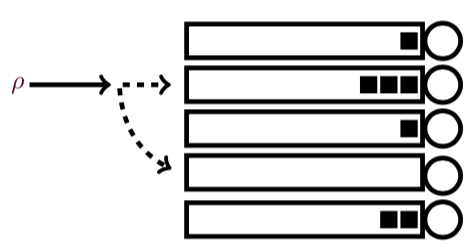
\includegraphics[width=\linewidth]{supermarket}}
    &\mpage{.35}{Arrival at each server $\rho$.
      \begin{itemize}
      \item Sample $d-1$ other queues. 
      \item Allocate to the shortest queue
      \end{itemize}
      Service rate=$1$.
      }
  \end{tabular}\bigskip
  
  \begin{center}
    \begin{tabular}{|c|c|c|c|c|}
      \hline
      &$N=10$&$N=20$&$N=50$&$N=100$\\\hline
      Mean Field	 & 2.3527	 & 2.3527	 & 2.3527	 & 2.3527	 \\
      $1/N$-expansion	 & 2.7513	 & 2.5520	 & 2.4324	 & 2.3925	 \\
      $1/N^2$-expansion	 & 2.8045	 & 2.5653	 & 2.4345	 & 2.3930	  \\
      Simulation	 & 2.8003	 & 2.5662	 & 2.4350	 &
                                                                           2.3931
      \\\hline
    \end{tabular}
  
    $SQ(2)$: \textbf{Steady-state average queue length} ($\rho=0.9$).
  \end{center}

\end{frame}

\begin{frame}{How does the expected queue length evolve with time?}
  
  \begin{tabular}{@{}c@{}c@{}}
    \begin{tabular}{@{}c@{}}
      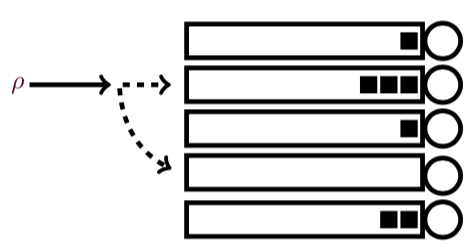
\includegraphics[width=.3\linewidth]{supermarket}
    \end{tabular}
    &
      \begin{tabular}{@{}c@{}}
        \only<1>{\includegraphics[width=.7\linewidth]{twoChoice_transient_N1000_rho90}}%
        \only<2>{\includegraphics[width=.7\linewidth]{twoChoice_transient_N10_rho90}}%
        \only<3>{\includegraphics[width=.7\linewidth]{twoChoice_refRefTransient_N10_rho90}}
      \end{tabular}
  \end{tabular}

  \pause\pause \footnotesize Remark about computation time :
  \begin{itemize}
  \item 10min/1h (simulation $N=1000$/$N=10$), C++ code. Requires many
    simulations, confidence intervals,...
  \item $80$ms (mean field), $700$ms ($1/N$-expansion), $9$s
    ($1/N^2$-expansion), Python \texttt{numpy}
  \end{itemize}

\end{frame}

\begin{frame}{Analysis of the computation time}
  For the numerical examples of $SQ(2)$, I used a bounded queue size
  $d$.
  \begin{center}
    \begin{tabular}{@{}c|c}
      \includegraphics[width=.45\linewidth]{jsqD_computationTime_order1_steadyState}
      &\includegraphics[width=.45\linewidth]{jsqD_computationTime_order2_steadyState}\\
      Time to compute the $1/N$-expansion
      &Time to compute the $1/N^2$-expansion\\\hline
    \end{tabular}\\
    Analysis of the computation time (Python numpy implementation)
  \end{center}
\end{frame}

\section{Conclusion and Open Questions}

\begin{frame}{Recap and extensions}
  For a mean field model with four differentiable drift
  \begin{align*}
    \esp{X(t)} = x(t) + \frac{V(t)}{N} + \frac{A(t)}{N^2}+ \dots 
  \end{align*}
  \begin{itemize}
  \item We can build expansion in $1/N$ 
  \end{itemize}
  % \pause
  \bigskip
  From a computational point of view:
  \begin{itemize}
  \item The $1/N$-term involves $d^2$ linear equations.
  \item The $1/N^2$-term involves $d^4$ linear equations.
  \item Most of the gain seems to come from the $1/N$-term. 
  \end{itemize}
\end{frame}

\begin{frame}{Some References}

  
  \begin{center}
    Paper (simulation, slides) is reproducible!
    \url{https://github.com/ngast/sizeExpansionMeanField/}
    \vspace{1cm}
    \texttt{nicolas.gast@inria.fr}\\ \bigskip
    \url{http://mescal.imag.fr/membres/nicolas.gast}
  \end{center}

  \bigskip
  
  \begin{itemize}
      \item \tiny \blue{A Refined Mean Field Approximation} by Gast
        and Van Houdt. SIGMETRICS 2018 (best paper award)
      \item \blue{Size Expansions of Mean Field Approximation:
          Transient and Steady-State Analysis} Gast, Bortolussi,
        Tribastone
      \item \blue{Expected Values Estimated via Mean Field Approximation
          are O(1/N)-accurate} by Gast. SIGMETRICS 2017.
      \item \url{https://github.com/ngast/rmf_tool/}
      \end{itemize}
    \end{frame}


\end{document}
